\documentclass{article}
\usepackage[a4paper, total={8.5in, 11in}, margin=0.5in]{geometry}
\usepackage{multicol}
\usepackage{parskip}
\usepackage{graphicx}

\title{
Spider 880 \\
\large Failure of 880 Machines in REBS Working Environment \\
A Comprehensive Report
}
\author{From the Desk of the Spider Computing Infrastructure Efficacy Working Group}
\date{}

\begin{document}
	\maketitle


\section{Introduction}
The Spider 880 Desktop Home Computer model has shown remarkable performance in Plinkett's Key Four consumer areas. If it is to continue to meet investor expectations, key sales issues must be addressed with Spider Computing's ongoing collaboration with the Rorik's End's Bureau of Sabotage (REBS). REBS currently claims dominion of a number of stressor points on both hardware and software simultaneously.

After extensive testing with multiple focus groups within the REBS Tetartoid, we present our findings for your consideration.

\begin{multicols}{2}
[
\section{Summary}
]
\subsection{Errors Experienced}
\subsubsection{SPN Violations}
The standout bug present amongst the 880s assigned to REBS personnel is their seemingly hindered SPN filters. 880s are able to display content that would normally be blocked on other networks, such as Gore, Slander, or Copyright Infringement.

\begin{center}
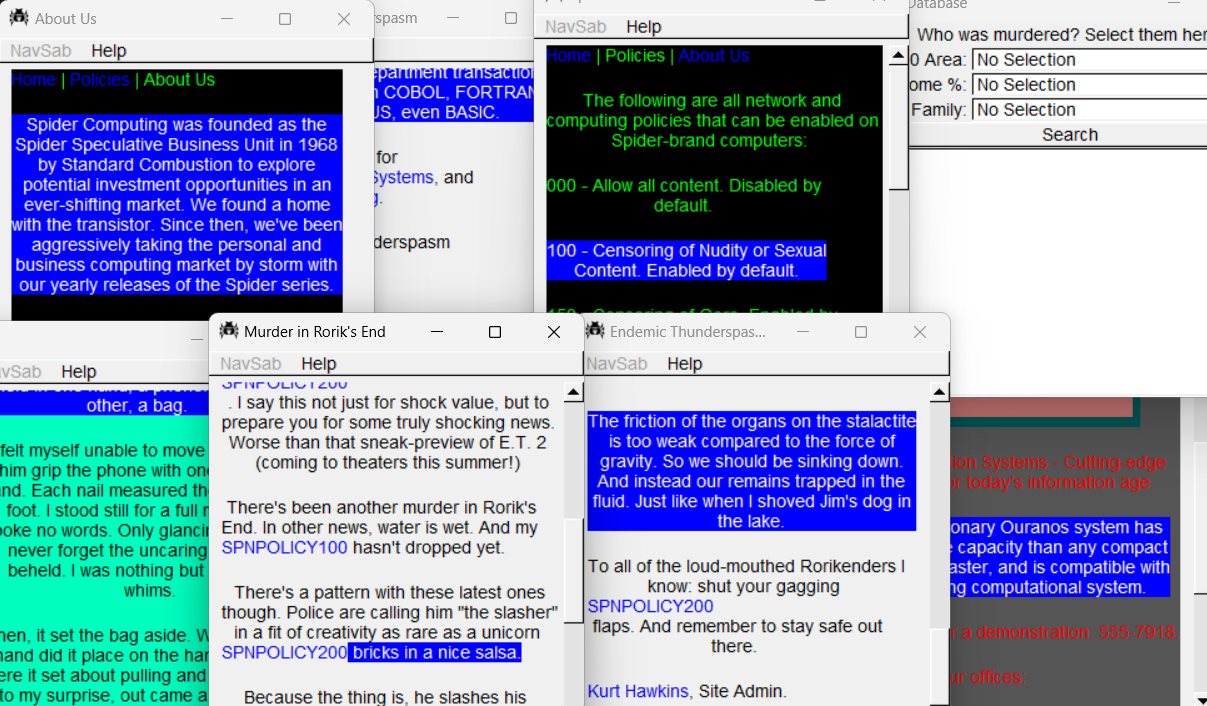
\includegraphics[scale=0.25]{spnpolicy.png}
\end{center}

REBS Management highlighted this as a priority issue: it is severely impacting employee morale. News of murders in Rorik's End in proximity to REBS employees is leading to decreased productivity.

\subsubsection{Security Vulnerabilities}
Worse among these errors is that any user in the system is granted level 2 permissions, which allows them access to the entirety of the REBS link to the Rorik's End Citizen Database. Seeing as how REBS is already under suit pertaining to HIPAA violations, a fix has been recommended to their technical support team. We have yet to hear back.

\begin{center}
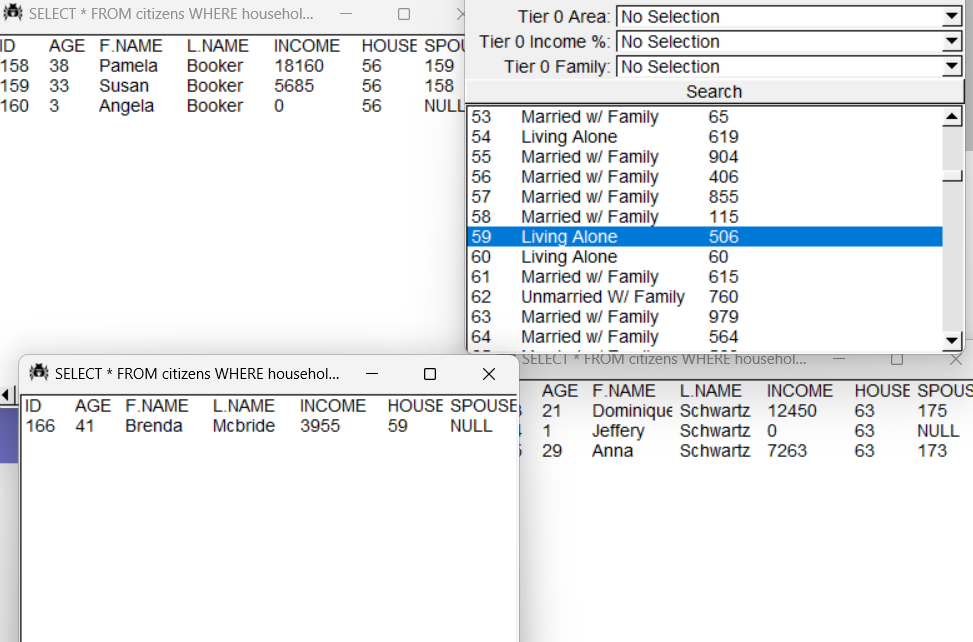
\includegraphics[scale=0.25]{database.png}
\end{center}

\subsubsection{Memory Leaks}
As documented by some REBS employees, 760s experience a huge amount of memory leaks during usage. The problem is reduced among REBS 880s, but they still experience the problem. The issue has currently been narrowed to some sort of interference from the 880 keyboard interrupt event spilling over into windows that have been marked by SC Secure-Lock(tm) as input friendly.

\begin{center}

\includegraphics[scale=0.1]{AH49CI.png}
\end{center}

\subsection{Likely Stressors}
Potential solutions for any of these problems are outlined in Section 4. 

This forgets the main issue, however: REBS poses many unique management and technical problems. Their focus on rapid processing of communication requires reliable engineering that is more suited to our enterprise class computing models. The 880s are, by comparison, newer than series like the 700s which have seen years of support and upgrades. With further hardware upgrades, the upcoming 900 would easily be able to meet the needs of REBS employees and management. It is therefore imperative that these needs be communicated to REBS executives before any additional requests or purchases are processed.
\end{multicols}
\end{document}